%% ─────────────────────────────────────────────────────────────────────────────
%%  Clasificación de conos y ejemplos de ENO
%% ─────────────────────────────────────────────────────────────────────────────
\section{Clasificación de conos}

\begin{frame}{Tipos de conos en un ENO}
\framesubtitle{Propiedades geométricas que determinan el comportamiento de BV}

\begin{block}{}
\centering
\large Algunos tipos de conos
\end{block}

\begin{itemize}
    \item \textbf{Conos normales}
    \begin{itemize}
        \item[$\ast$] \textbf{Normal:} existe $M>0$ tal que
            $0 \le x \le y \Rightarrow \|x\| \le M\|y\|$.
        \item[$\ast$] \textbf{Extendible:} existe $x^{*}\in \Xp^{*}$ y $\alpha>0$
            tal que $x^{*}(x)\ge\alpha\|x\|$ para todo $x\in\Xp$.
    \end{itemize}
    \item \textbf{Conos no normales}
    \begin{itemize}
        \item[$\ast$] \textbf{Generador:} $X = \Xp - \Xp$, es decir, todo
            $x\in X$ se escribe como $x=\alpha-\beta$ con $\alpha,\beta\in\Xp$.
        \item[$\ast$] \textbf{Sólido:} $\operatorname{int}(\Xp)\ne\emptyset$.
    \end{itemize}
\end{itemize}

% IDEA ORAL: Recordar que estas propiedades no son técnicas por sí mismas,
% sino que cada una tiene una consecuencia concreta sobre las funciones BV.

\end{frame}

%──────────────────────────────────────────────────────────────────────────────

\begin{frame}{Relaciones entre tipos de conos}
\framesubtitle{¿Qué implica qué?}

\begin{columns}[c]
\column{.60\textwidth}
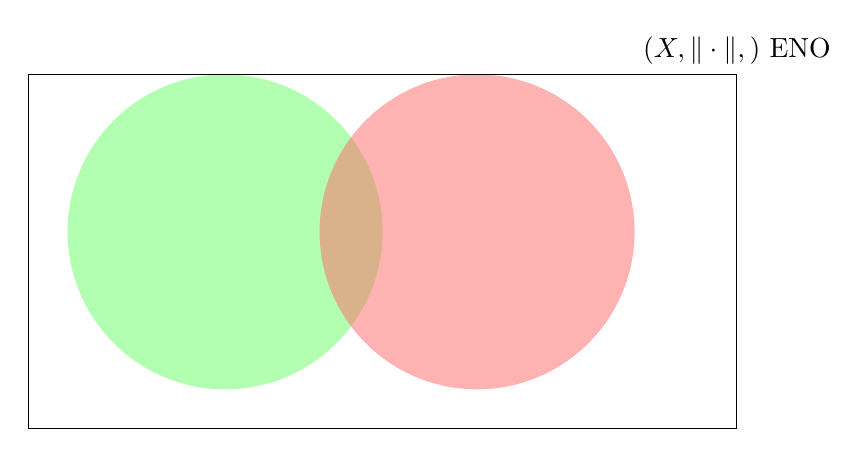
\begin{tikzpicture}
    \begin{scope}[shift={(3cm,-3cm)}, fill opacity=0.5]
        \def\Gcirc{(0.5,0) circle (2cm)}
        \def\Ncirc{(0:3.7cm) circle (2cm)}
        \fill[green!60!white] \Gcirc;
        \fill[red!60!white]   \Ncirc;
        \draw (-2,-2.5) rectangle (7,2)
              node[text=black,above,fill opacity=1,text opacity=1]
              {$(X,\|\cdot\|,\Xp)$ ENO};
    \end{scope}
\end{tikzpicture}

\column{.38\textwidth}
\begin{itemize}
    \item \textcolor{green!70!black}{Verde:} cono generador
    \item \textcolor{red!70!black}{Rojo:} cono normal
    \item \textcolor{brown}{Intersección:} generador y normal
\end{itemize}

\medskip
\small
\textbf{Sólido} $\Rightarrow$ generador,
pero no al revés.

\end{columns}

\end{frame}

%──────────────────────────────────────────────────────────────────────────────

\begin{frame}{Ejemplo 1: ENO con cono normal}
\framesubtitle{$C^1_{\mathbb{R}}[a,b]$ con la norma del supremo}

\begin{block}{}
Sea $C_{\mathbb{R}}^{1}[a,b]$ con
$\|f\|_{\infty} = \sup_{x\in[a,b]}|f(x)|$
y el cono $\Xp = \{f\in C_{\mathbb{R}}^{1}[a,b] : f(x)\ge 0\}$.

$(C_{\mathbb{R}}^{1}[a,b],\|\cdot\|_{\infty},\Xp)$ es un ENO y $\Xp$ es \textbf{normal}.
\end{block}

\begin{columns}
\column{.58\textwidth}
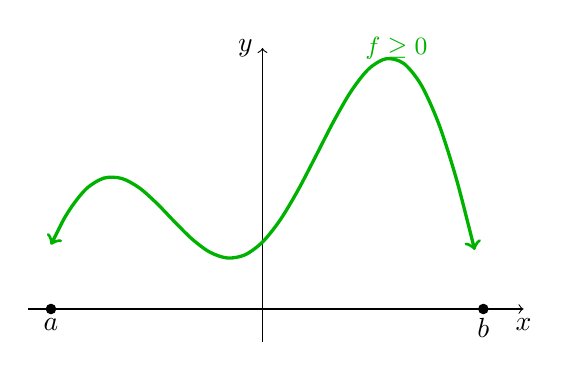
\begin{tikzpicture}[scale=0.85]
    \draw[->] (-3.5,0) -- (3.9,0) node[below] {$x$};
    \draw[->] (0,-0.5) -- (0,3.9) node[left] {$y$};
    \draw[smooth,<->,domain=-3.16:3.17,color=green!70!black,very thick]
        plot (\x,{sin(\x r)*(\x+1)+1});
    \node at (2,3.9) {\small\textcolor{green!70!black}{$f\ge 0$}};
    \draw[fill] (-3.16,0) circle (0.07) node[below]{$a$};
    \draw[fill] (3.3,0) circle (0.07) node[below]{$b$};
\end{tikzpicture}

\column{.40\textwidth}
\textbf{Consecuencia:} \\[4pt]
$0\le f\le g \Rightarrow \|f\|_\infty\le\|g\|_\infty$.

\medskip
Las sucesiones crecientes acotadas convergen.
\end{columns}

\end{frame}

%──────────────────────────────────────────────────────────────────────────────

\begin{frame}{Ejemplo 2: ENO con cono \textbf{no} normal}
\framesubtitle{$C^1_{\mathbb{R}}[0,1]$ con la norma $\|\cdot\|_\infty+\|\cdot'\|_\infty$}

\begin{block}{}
Sea $C_{\mathbb{R}}^{1}[0,1]$ con
$\|f\| = \|f\|_\infty + \|f'\|_\infty$
y $\Xp = \{f\in C_{\mathbb{R}}^{1}[0,1]: f(x)\ge 0\}$.

$\Xp$ \textbf{no es normal}.
\end{block}

\begin{columns}
\column{.55\textwidth}
\begin{tikzpicture}[scale=0.8]
    \draw[->] (-3.5,0) -- (3.9,0) node[below]{$x$};
    \draw[->] (0,-0.5) -- (0,3.9) node[left]{$y$};
    \draw[smooth,<->,domain=-3.16:3.17,color=green!70!black,very thick]
        plot (\x,{sin(\x r)+1});
    \node at (-0.5,0.5){\small\textcolor{green!70!black}{$f_n$}};
    \draw[->,color=MyTeal] (-3.16,2) -- (3.3,2) node[below]{$\bar{2}$};
    \draw[fill] (-3.16,0) circle (0.07) node[below]{$0$};
    \draw[fill] (3.3,0) circle (0.07) node[below]{$1$};
\end{tikzpicture}

\column{.43\textwidth}
$f_n(t)=\sin(2\pi n t)+1$.

\medskip
$0\le f_n\le\bar{2}$, pero
\[
\|f_n\| = 1 + 2\pi n \to\infty.
\]

La norma no está controlada por el orden.
\end{columns}

\end{frame}
